\chapter*{Lecture 10}
\begin{recall}{}{}
\begin{itemize}
\item Solution strategy for mathematical modelling problems
\item Examples Mathematical modelling
\end{itemize}
\end{recall}






\textbf{Terminal velocity of a falling object :}\\
A small sphere is released in a fluid which has a density of $\rho_f$. The mass and volume of the sphere is $m$ and $V$, respectively. Knowing the gravitational acceleration, $g$, and the drag coefficient, $k$, find:
\begin{itemize}
\item The velocity of the sphere $U(t)$
\item The terminal velocity, $U_{terminal}$
\end{itemize}
\begin{enumerate}
\item \textbf{Problem statement}

\begin{minipage}{0.6\textwidth}
\begin{itemize}
\item Pictorial representation:
\item Variables: $U(t)$, $t$
\item Parameters: $m$, $V$, $\rho_f$, $g$, $k$
\end{itemize}
\end{minipage}
\hspace{0.05\textwidth}
\begin{minipage}{0.25\textwidth}
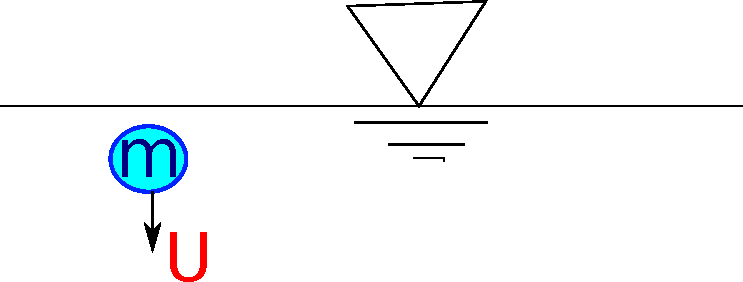
\includegraphics[width=\textwidth]{figs/terminalVelocity.pdf} 
\end{minipage}
\item \textbf{Formulate mathematical model:} (It's a good idea to set up a coordinate system as the velocity and forces have a direction!)\\
\begin{itemize}
\item Physical law: conservation of momentum (Newton's second law)
\item Mathematical expression: $m\frac{dU}{dt}=\sum F$
\item Find the net force on the falling object. We consider:
\begin{itemize}
\item Gravity force: $F_g=mg$
\item Buoyancy force: $F_b=\rho_f g V$
\item Drag force: $F_d = k U$
\end{itemize}
The net force is then:
\begin{equation}
\sum F=F_g-F_b-F_d=mg-\rho_f g V-kU
\end{equation}
\item The ODE is:
\begin{equation}
m\frac{dU}{dt}=mg-\rho_f g V-kU
\end{equation}
\item Write in standard form:
\begin{equation}
\frac{dU}{dt}+\frac{k}{m}U=g-\frac{\rho_f g V}{m}
\end{equation}
For simplicity, we replace $P=\frac{k}{m}$ and $Q=g-\frac{\rho_f g V}{m}$ to obtain:
\begin{equation}
\frac{dU}{dt}+PU=Q
\end{equation}
\end{itemize}
\item \textbf{Solve the ODE}: It is a linear equation! We find the integrating factors (denoted here at $U^*$ to avoid conflicts with the velocity!!!)
\begin{equation}
U^*=e^{\int P dt}=e^{k/m\int dt}=e^{kt/m}
\end{equation}
With the integrating factor, we end up with a simpler ODE to solve:
\begin{equation}
\frac{d}{dt}\left[U^*U\right]=U^*Q
\end{equation}
\begin{equation}
U^*U = \int U^*Q\,dt+C=Q\int  e^{kt/m} dt+C=Q\frac{m}{k}e^{kt/m}+C
\end{equation}
Or:
\begin{equation}
U =\frac{Q\frac{m}{k}e^{kt/m}+C}{e^{kt/m}}=Q\frac{m}{k}+\frac{C}{e^{kt/m}}
\end{equation}
 Apply IC: at $t=0$, $U(0)$
\begin{equation}
0 =Q\frac{m}{k}+C \qquad or \qquad C=\frac{-m}{k}Q
\end{equation}
The final solution is then:
\begin{equation}
U =\frac{m}{k}Q-\frac{m}{k}Q{e^{-kt/m}}=\frac{m}{k}Q\left(1-e^{-kt/m}\right)
\end{equation}
\item Application (find terminal velocity): Terminal velocity is obtained by a falling object when all the forces on the body cancel out: $\sum F=0$. Or, when $\frac{dU}{dt}=0$.

Using the final solution, we find:
\begin{equation}
\frac{dU}{dt}=Q\left(e^{-kt/m}\right)=0
\end{equation}
At what time will we reach a terminal velocity?

\end{enumerate}

\begin{center}
\noindent\rule{4cm}{0.4pt}
\end{center}

\begin{testv}{Electric circuits}{}
\begin{itemize}
\item The voltage drop $E_r$ across a resistor is proportional to the instantaneous current, $I$:
\begin{equation}
\boxed{E_r = RI}
\end{equation}
where the constant of proportionality $R$ is the resistance of the resistor. The current $I$ is measured in amperes, the resistance $R$ in ohms and the voltage, $E_r$ in volts. 
\item A inductor opposes a change in current. The voltage drop across an inductor is proportional to the instantaneous time rate of change of the current.
\begin{equation}
\boxed{E_L = L\frac{dI}{dt}}
\end{equation}
where $L$ is the inductance of the inducer measured in henrys and $t$ is time in seconds.
\item A capacitor is an element that stores energy. The voltage drop $E_c$ across a capacitor is proportional to the instantaneous electric charge $Q$ on the capacitor:
 \begin{equation}
\boxed{E_c = \frac{1}{C}Q}
\end{equation}
where $C$ is the capacitance and is measured in farads. The charge $Q$ is measured in coulombs since:
 \begin{equation}
I(t) = \frac{dQ}{dt}
\end{equation}
therefore, we can write:
 \begin{equation}
E_c = \frac{1}{C}\int^t_{t_0}I(t*) dt*
\end{equation}
\end{itemize}
\textbf{Kirchoff's voltage law}\\
The algebraic sum of all the instantaneous voltage drops around any closed loop is zero.

\end{testv}

\updateinfo[October 1, 2018]
